% Appendix A

\chapter{Appendix} % Main appendix title

\label{AppendixA} % For referencing this appendix elsewhere, use \ref{AppendixA}

\lhead{Appendix A. \emph{Appendix A}} % This is for the header on each page - perhaps a shortened title
\begin{figure}[ht]
	\centering
		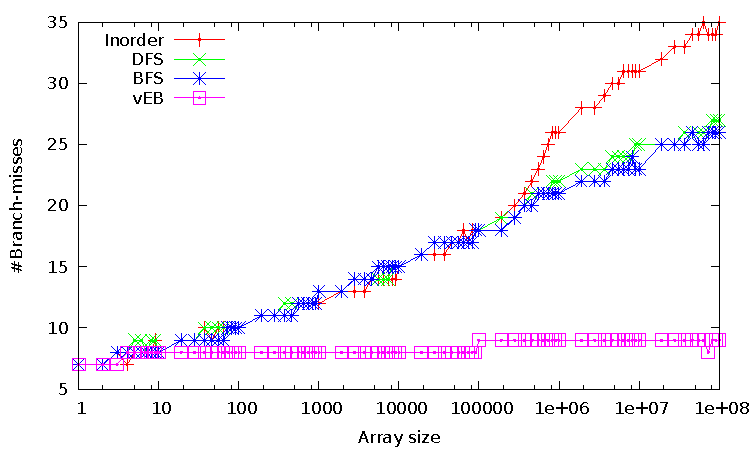
\includegraphics[width=\textwidth]{./Appendices/Figures/Project1/Branch_misses-Putty.pdf}
		\rule{35em}{0.5pt}
	\caption[Branch misses]{
	Branch misses from llama01 - project 1
	}
	\label{fig:Branch_misses_p1putty}
\end{figure}
\begin{figure}[ht]
	\centering
		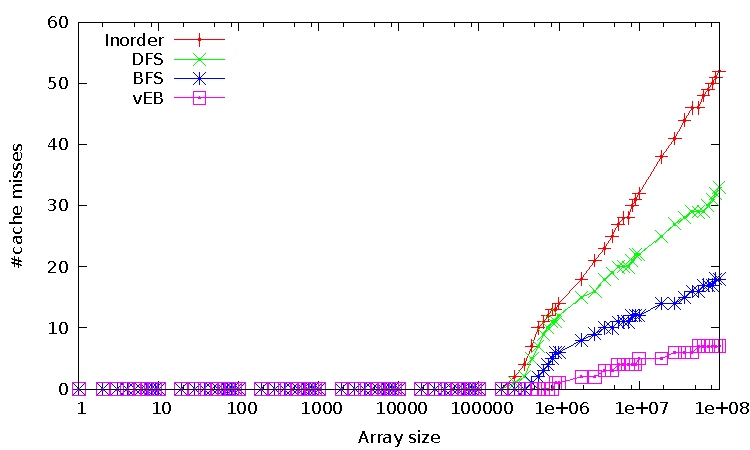
\includegraphics[width=\textwidth]{./Appendices/Figures/Project1/Cache_misses-putty.pdf}
		\rule{35em}{0.5pt}
	\caption[Cache misses]{
	Cache misses from llama01 - project 1
	}
	\label{fig:Cache_misses_p1putty}
\end{figure}
\begin{figure}[ht]
	\centering
		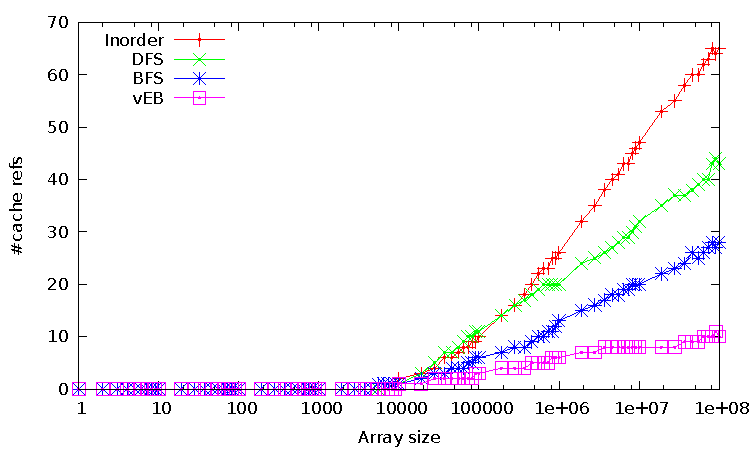
\includegraphics[width=\textwidth]{./Appendices/Figures/Project1/Cache_refs-Putty.pdf}
		\rule{35em}{0.5pt}
	\caption[Cache refs]{
	Cache refs from llama01 - project 1
	}
	\label{fig:Cache_refs_p1putty}
\end{figure}
\begin{figure}[ht]
	\centering
		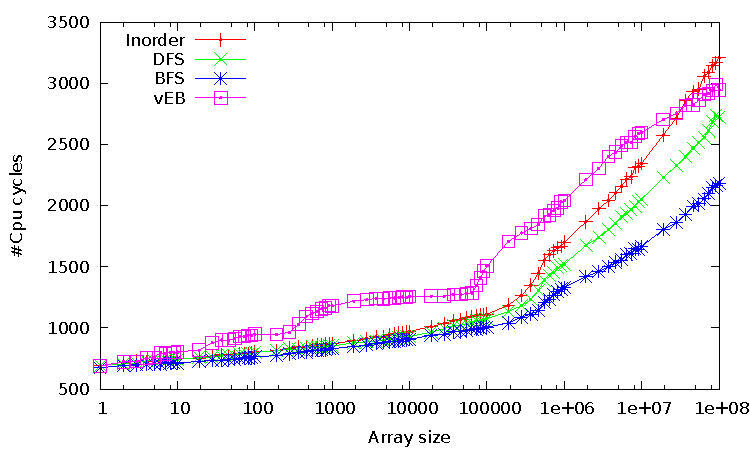
\includegraphics[width=\textwidth]{./Appendices/Figures/Project1/Cpu_cycles-Putty.pdf}
		\rule{35em}{0.5pt}
	\caption[Cpu cycles]{
	Cpu cycles from llama01 - project 1
	}
	\label{fig:Cpu_cycles_p1putty}
\end{figure}
\begin{figure}[ht]
	\centering
		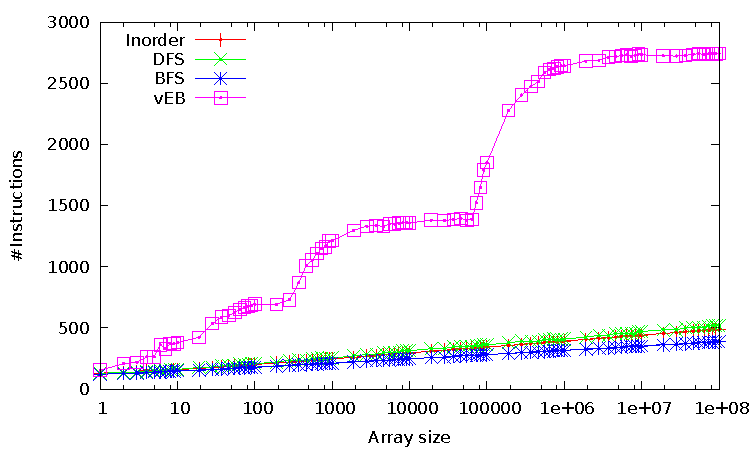
\includegraphics[width=\textwidth]{./Appendices/Figures/Project1/Instructions-Putty.pdf}
		\rule{35em}{0.5pt}
	\caption[Instructions]{
	Instructions from llama01 - project 1
	}
	\label{fig:Instructions_p1putty}
\end{figure}

\begin{figure}[ht]
	\centering
		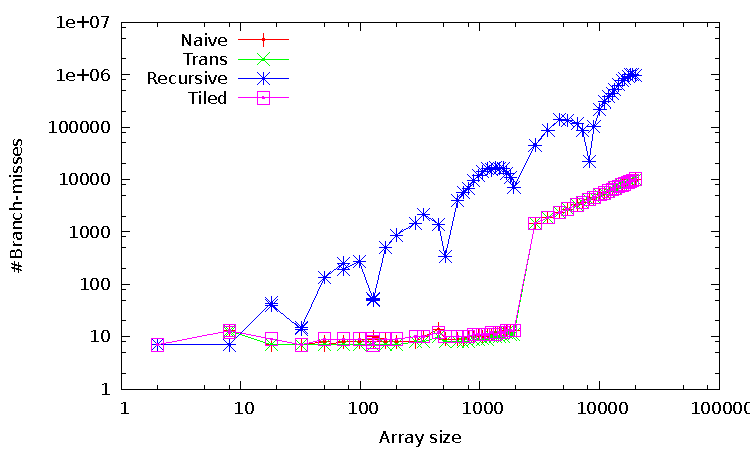
\includegraphics[width=\textwidth]{./Appendices/Figures/Project2a/Branch_misses_putty.pdf}
		\rule{35em}{0.5pt}
	\caption[Branch misses]{
	Branch misses from llama01 - project 2a
	}
	\label{fig:Branch_misses_p2putty}
\end{figure}
\begin{figure}[ht]
	\centering
		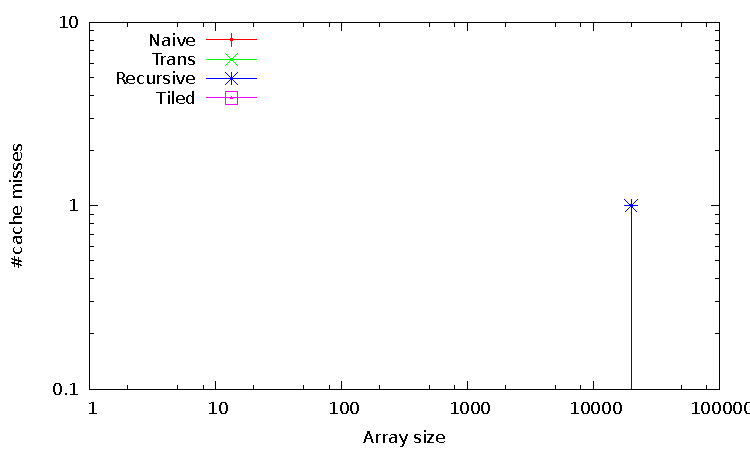
\includegraphics[width=\textwidth]{./Appendices/Figures/Project2a/Cache_misses_putty.pdf}
		\rule{35em}{0.5pt}
	\caption[Cache misses]{
	Cache misses from llama01 - project 2a
	}
	\label{fig:Cache_misses_p2putty}
\end{figure}
\begin{figure}[ht]
	\centering
		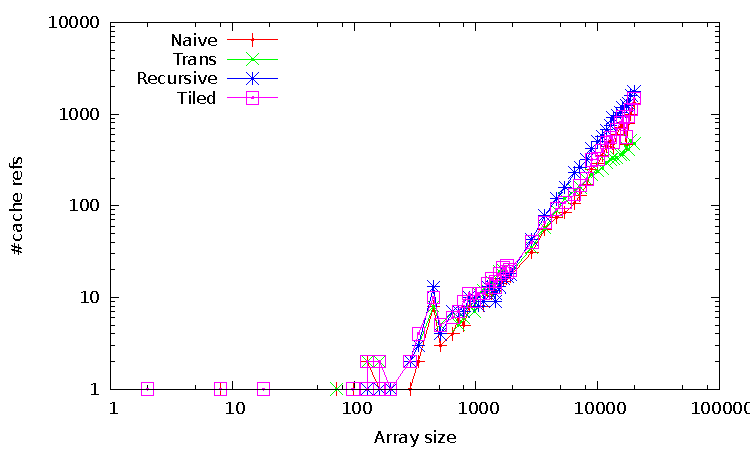
\includegraphics[width=\textwidth]{./Appendices/Figures/Project2a/Cache_refs_putty.pdf}
		\rule{35em}{0.5pt}
	\caption[Cache refs]{
	Cache ref from llama01 - project 2a
	}
	\label{fig:Cache_refs_p2putty}
\end{figure}
\begin{figure}[ht]
	\centering
		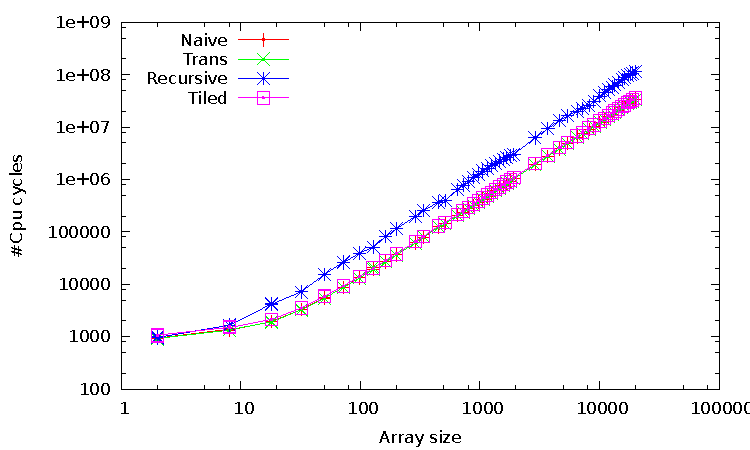
\includegraphics[width=\textwidth]{./Appendices/Figures/Project2a/Cpu_cycles_putty.pdf}
		\rule{35em}{0.5pt}
	\caption[Cpu cycles]{
	Cpu cycles from llama01 - project 2a
	}
	\label{fig:Cpu_cycles_p2putty}
\end{figure}
\begin{figure}[ht]
	\centering
		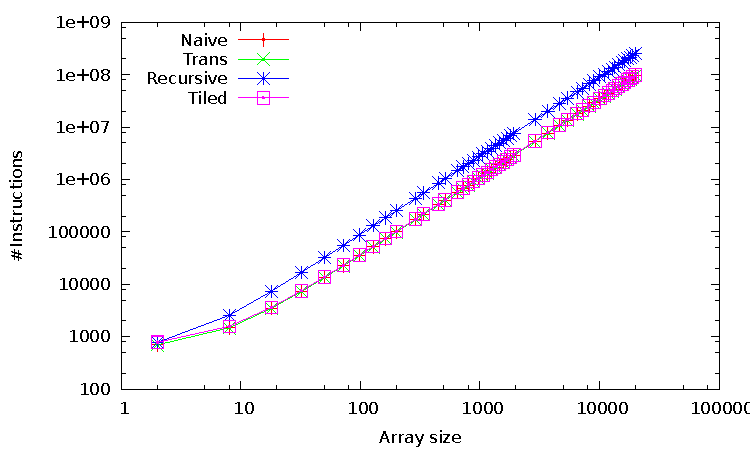
\includegraphics[width=\textwidth]{./Appendices/Figures/Project2a/Instructions_putty.pdf}
		\rule{35em}{0.5pt}
	\caption[Instructions]{
	Instructions from llama01 - project 2a
	}
	\label{fig:Instructions_p2putty}
\end{figure}

\begin{figure}[ht]
	\centering
		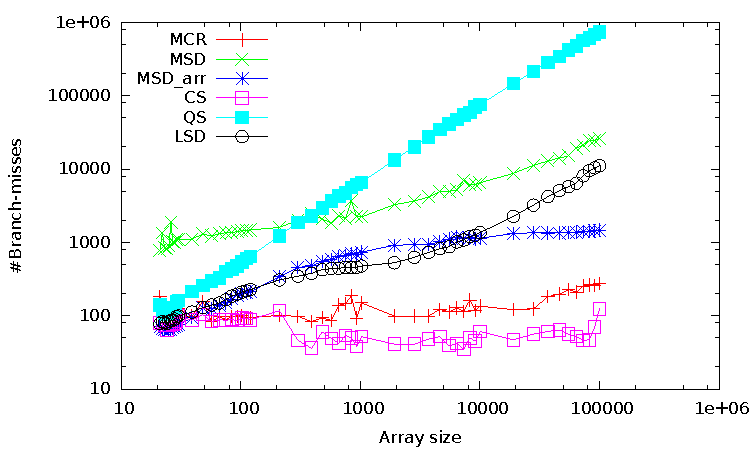
\includegraphics[width=\textwidth]{./Appendices/Figures/Project2b/Branch_misses.pdf}
		\rule{35em}{0.5pt}
	\caption[Branch misses]{
	Branch misses from llama01 - project 2b
	}
	\label{fig:Branch_misses_p2bputty}
\end{figure}
\begin{figure}[ht]
	\centering
		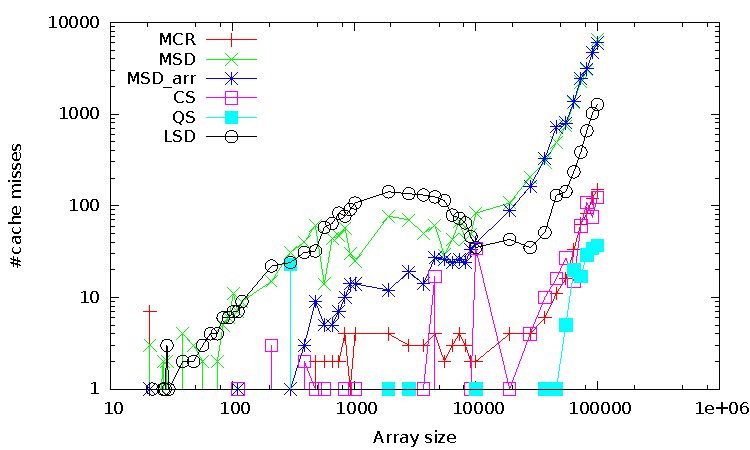
\includegraphics[width=\textwidth]{./Appendices/Figures/Project2b/Cache_misses.pdf}
		\rule{35em}{0.5pt}
	\caption[Cache misses]{
	Cache misses from llama01 - project 2b
	}
	\label{fig:Cache_misses_p2b_putty}
\end{figure}
\begin{figure}[ht]
	\centering
		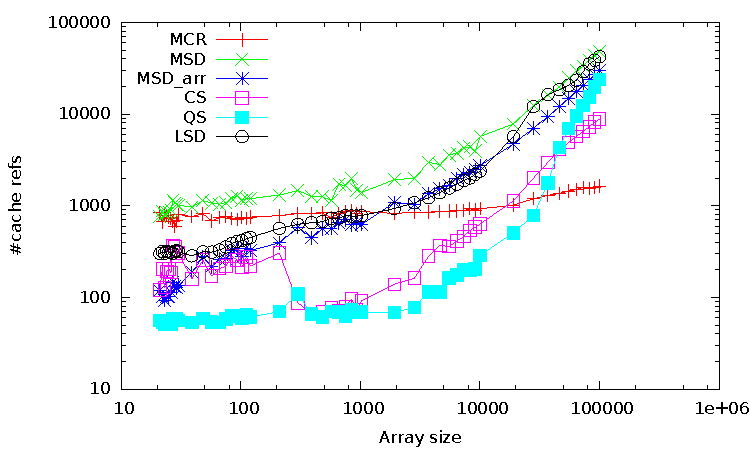
\includegraphics[width=\textwidth]{./Appendices/Figures/Project2b/Cache_refs.pdf}
		\rule{35em}{0.5pt}
	\caption[Cache refs]{
	Cache refs from llama01 - project 2b
	}
	\label{fig:Cache_refs_p2b_putty}
\end{figure}
\begin{figure}[ht]
	\centering
		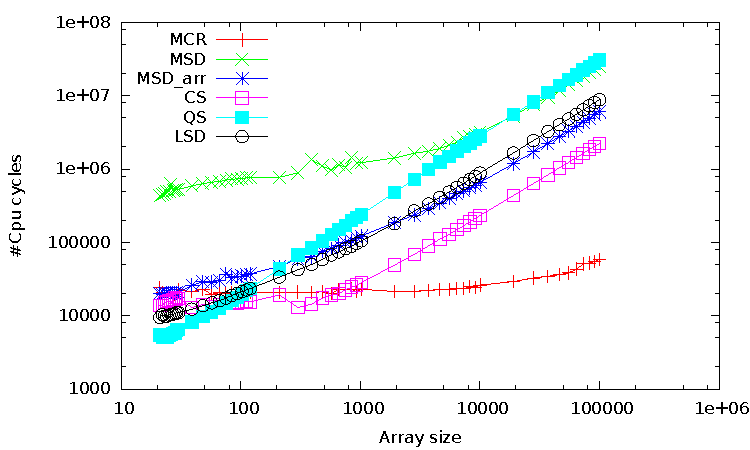
\includegraphics[width=\textwidth]{./Appendices/Figures/Project2b/Cpu_cycles.pdf}
		\rule{35em}{0.5pt}
	\caption[Cpu cycles]{
	Cpu cycles from llama01 - project 2b
	}
	\label{fig:Cpu_cycles_p2b_putty}
\end{figure}
\begin{figure}[ht]
	\centering
		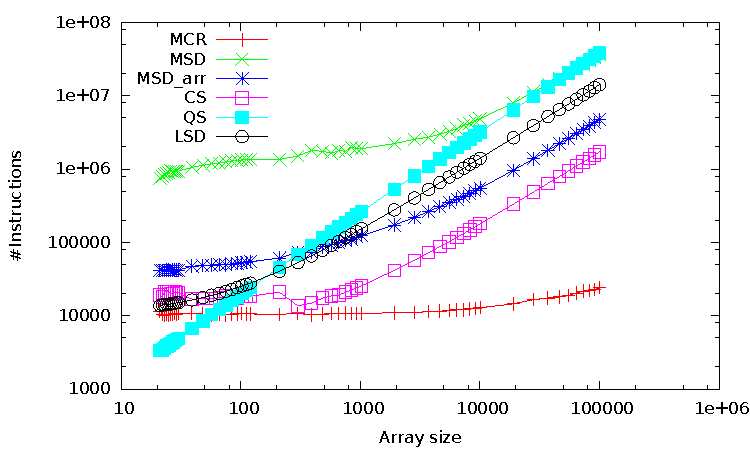
\includegraphics[width=\textwidth]{./Appendices/Figures/Project2b/Instructions.pdf}
		\rule{35em}{0.5pt}
	\caption[Instructions putty]{
	Instructions from llama01 - project 2b
	}
	\label{fig:Instructions_p2b_putty}
\end{figure}